\documentclass[12pt]{article}
\usepackage[a4paper,bindingoffset=0.2in,%
            left=1in,right=1in,top=1in,bottom=1in,%
            footskip=.25in]{geometry}
\usepackage{graphicx}
\usepackage{placeins}
\usepackage{float}
\usepackage{afterpage}

\author{Jan Witkowski s18749, Yoon Jongok s18349}
\title{HP Support System - Documentation}

\begin{document}
  \maketitle

  \section{Not Optimized Version}
  The process of servicing a broken HP laptop starts with a client reporting a damage by phone call.
  The customer service employee asks the serial number of the laptop and creates a ticket and adds it to the database.
  Then check the warranty.
  If the warranty is not valid, the company will notify the client about the expected cost of the repair and wait for the client’s decision for 7 days.
  If the client does not agree to the price or give the decision within 7 days, the process ends.
  
  If it is valid (or the customer agreed to the cost), the company sends a technician to evaluate the damage.
  If the damage can be fixed at the customer's place, the technician fixes it.
  Technician prepares an invoice and gives it to the client in case of invalid warranty, then the process ends.
  If it cannot be fixed at the client’s place, the technician will take the laptop to the repair center, and it will be sent back to the client after at most 30 days.
  If the warranty was not valid, an invoice will be sent to the client.
  
  When the laptop is available in the service point, it will be analyzed by a maintenance specialist in order to pinpoint the problem with it.
  If the warranty is valid, the laptop will be repaired for free.
  If not, after the problem is identified, the maintenance specialist will have to estimate the repair costs and notify it to the customer service.
  Then customer service prepares an invoice and sends it to the client.
  The client will get  the estimation and will have to make a decision – either to pay the repair costs or get his device back without repairs.
  He has 7 business days to make that decision.
  If he makes no decision, then the device will not be repaired.
  
  After the client decides to pay (or if the device repairs are covered by warranty), the maintenance specialist will repair the device and then test it.
  Then the client is notified that his/her device will be delivered within 7days.
  If the client decides not to pay for the repairs, the device will be sent back to the client.
  Then the process ends.

  \clearpage
  \subsection{Business Use case diagram}

  \FloatBarrier
  \begin{figure}[!htbp]
    \centering
    \def\svgwidth{\columnwidth}
    \input{business_usecase_diagram.pdf_tex}
    \caption{Business Use Case diagram}
  \end{figure}
  \FloatBarrier

  \subsection{Business analysis diagram}

  \FloatBarrier
  \begin{figure}[!htbp]
    \centering
    \def\svgwidth{\columnwidth}
    \scalebox{0.8}{\input{sequence_diagram.pdf_tex}}
    \caption{Business analysis diagram}
  \end{figure}
  \FloatBarrier

  \subsection{Bpmn diagram}

  \FloatBarrier
  \begin{figure}[!htbp]
    \centering
    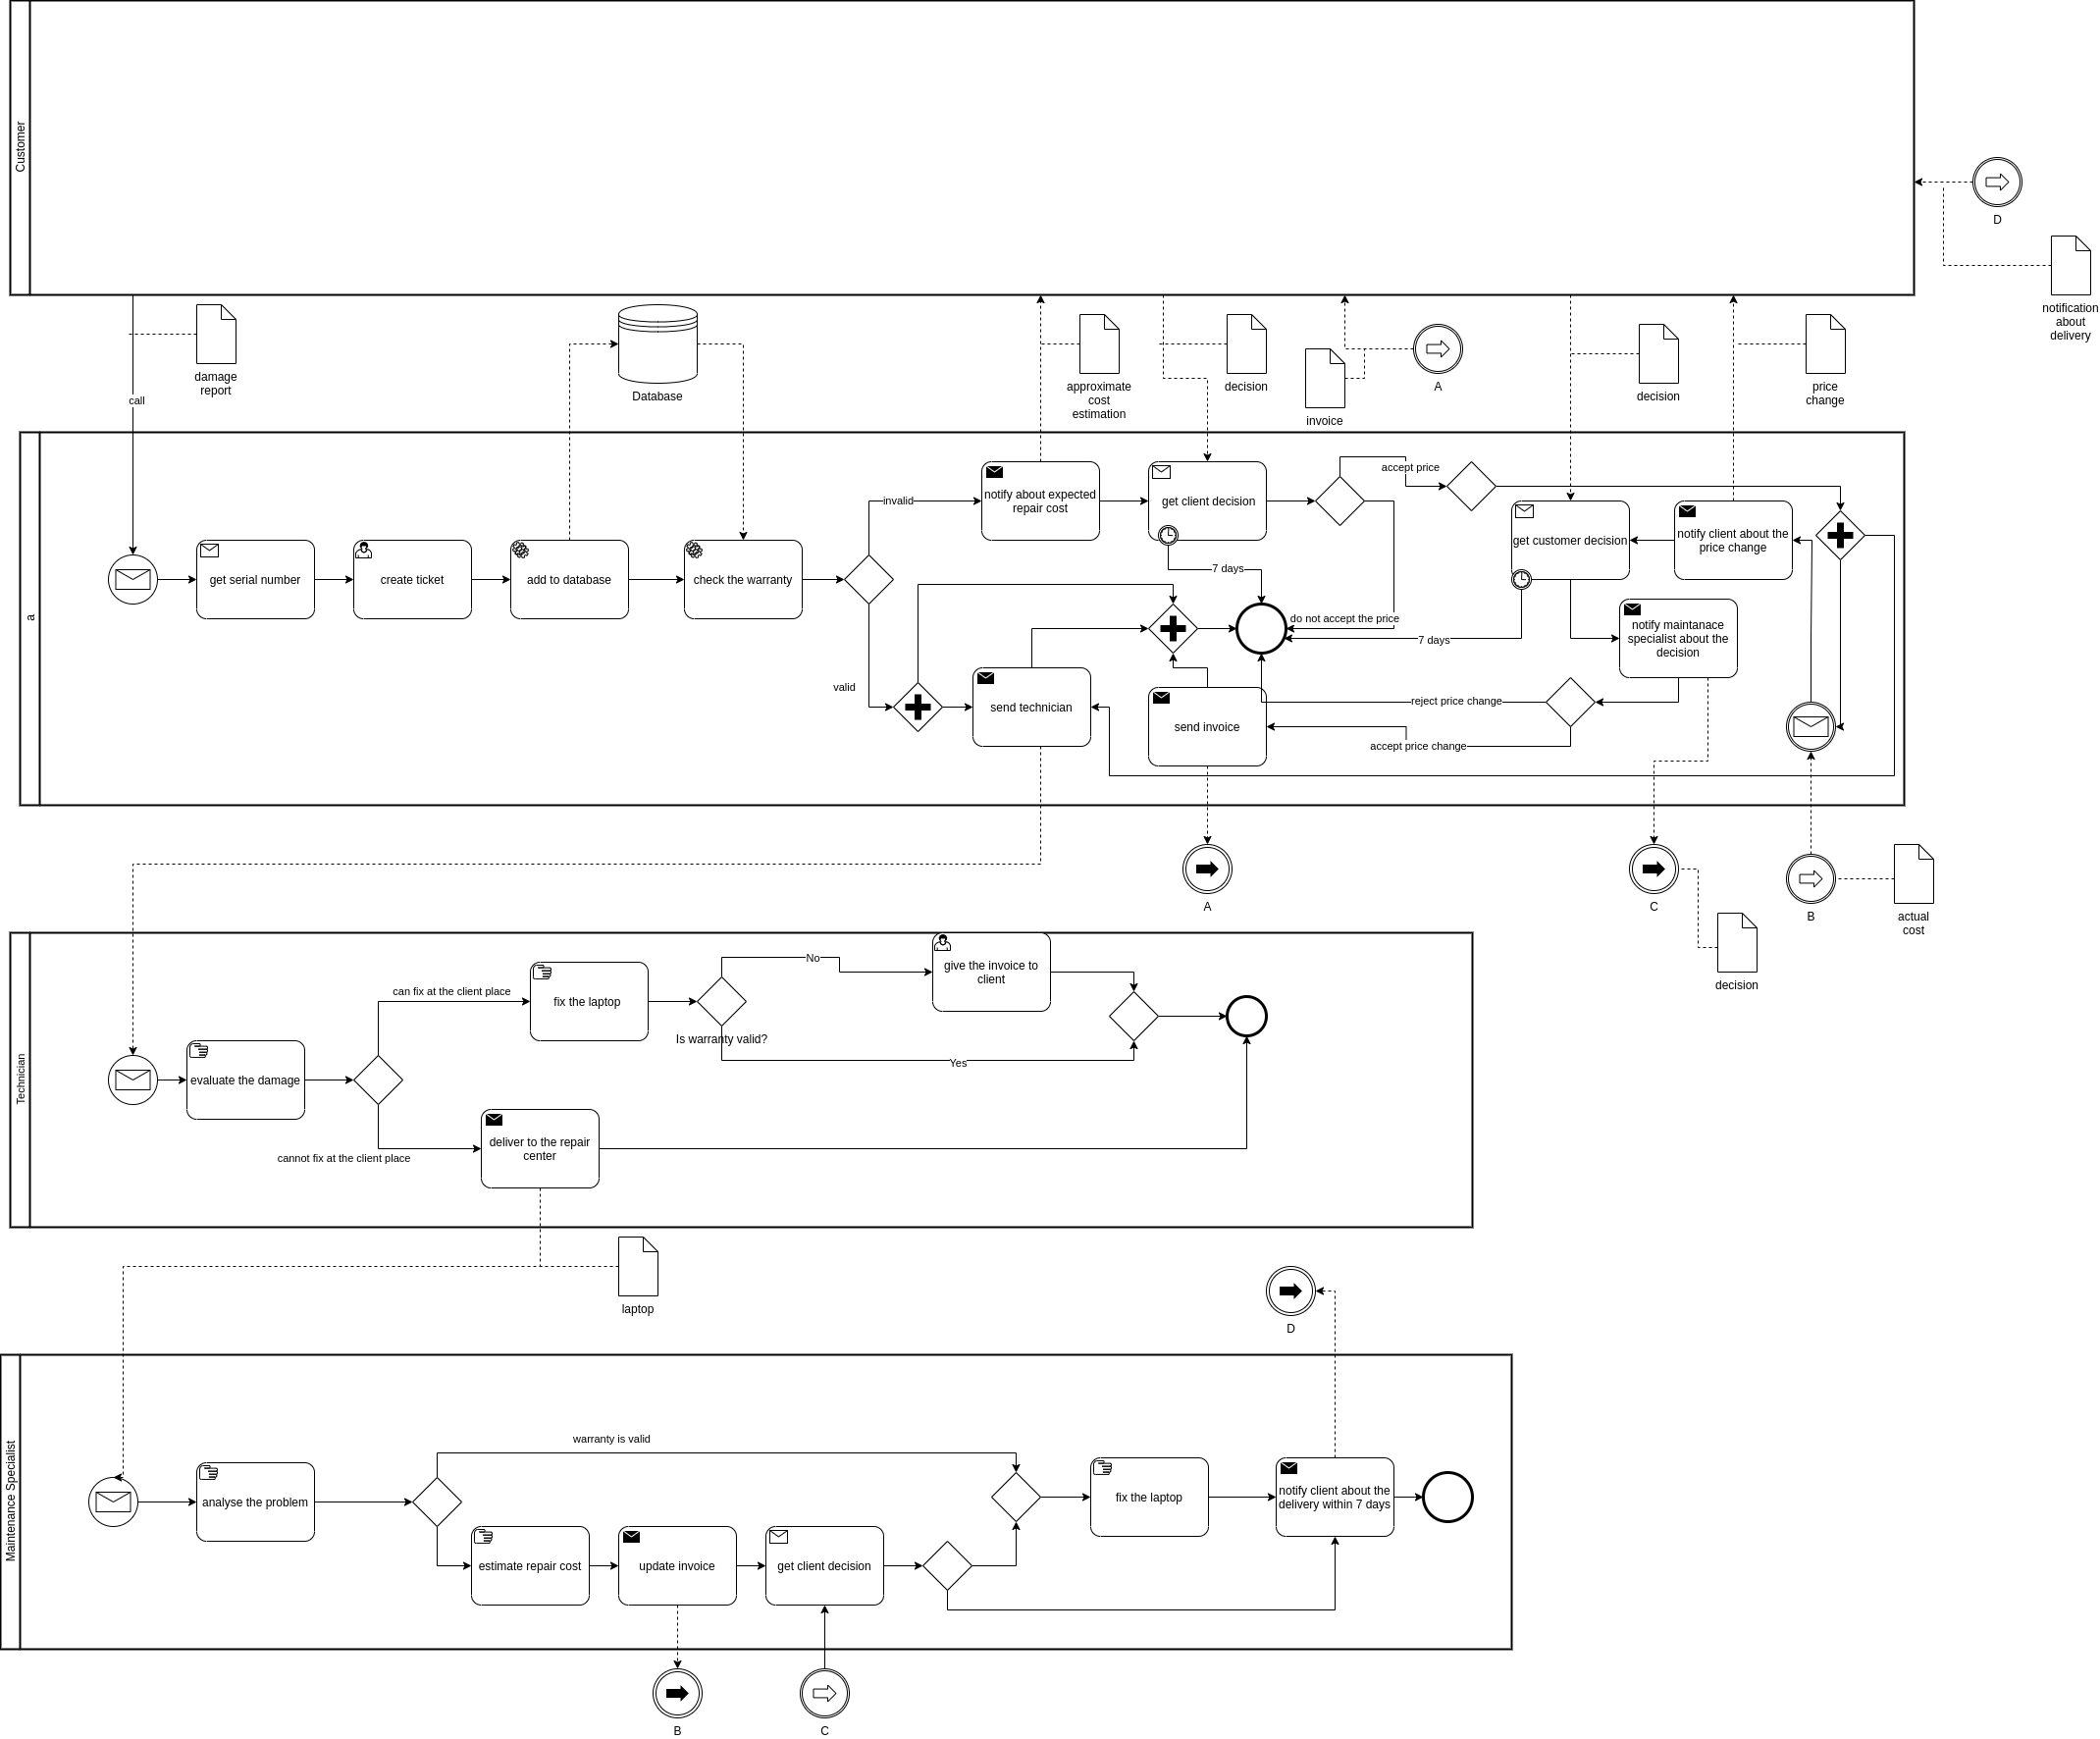
\includegraphics[width=1\textwidth]{bpmn_not_optimized.png}
    \caption{Bpmn diagram}
  \end{figure}
  \FloatBarrier

  \section{Optimized Version}

  The process of servicing a broken HP laptop starts with a client registering a repair request.
  The device details, as well as information about the warranty, are confirmed by the system.
  Repair requests will contain information about the observed damage, and client’s consent to the approximate cost calculated by the system (in case warranty is not valid).
  Then the request ticket will be added to the database.
  
  If the warranty is not valid, the system will automatically generate an invoice for the client and send it to him.
  
  If the damage can be fixed at the client’s place, a technician will be sent to fix the laptop and the process ends.
  
  If not, the delivery employee will be sent to pick up the laptop and he will deliver it to the repair center.
  
  When the laptop is available in the service point, it will be analyzed again by a maintenance specialist in order to pinpoint the problem with it and estimate the actual cost of the problem.
  If the cost is higher than the approximated one and there is no valid warranty, the client will be notified of the estimation and will have to make a decision – either to pay the repair costs or get his device back without repairs.
  He has 7 business days to make that decision.
  If he makes no decision, then the device will not be repaired.
  
  After the client decides to pay (or if the device repairs are covered by warranty), the maintenance specialist will repair the device.
  Then the client is notified that his/her device will be delivered within 7days.
  If the client decides not to pay for the repairs, the device will be sent back to the client.
  Then the process ends.


  \subsection{Bpmn diagram}

  \FloatBarrier
  \begin{figure}[!htbp]
    \centering
    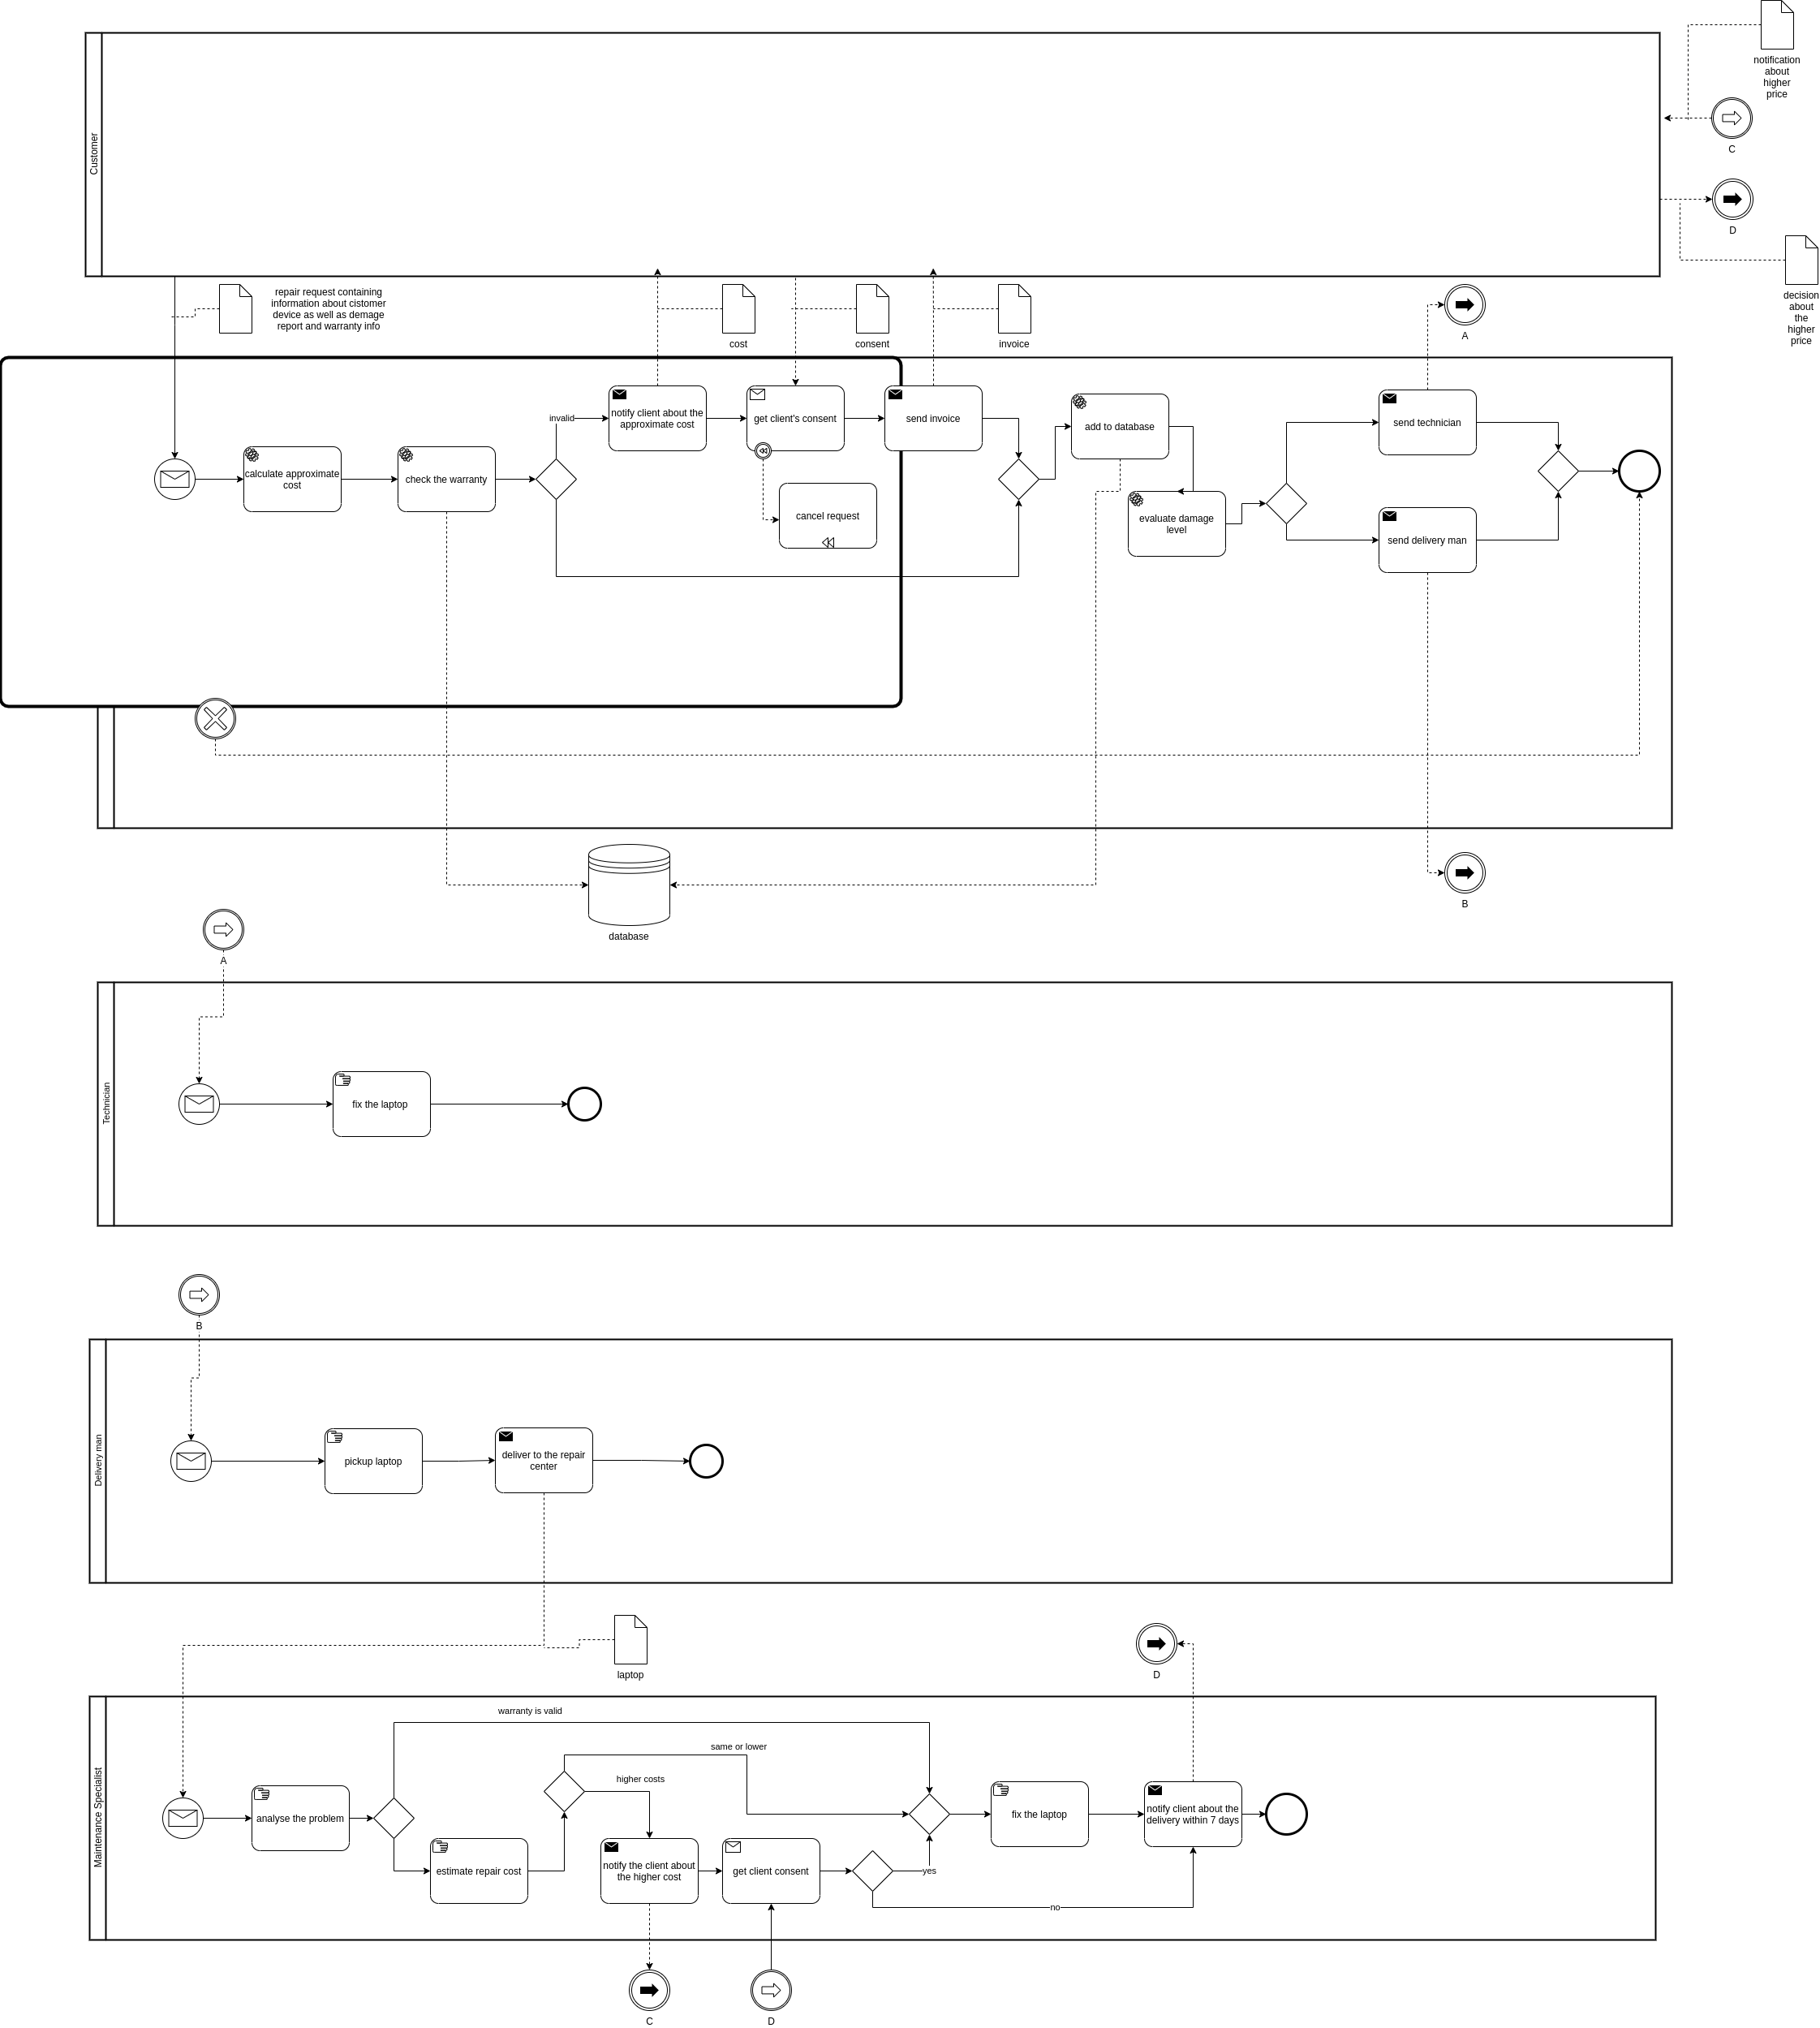
\includegraphics[width=1\textwidth]{bpmn_optimized.png}
    \caption{Bpmn diagram}
  \end{figure}
  \FloatBarrier

  \subsection{Use Case diagram}
  \FloatBarrier
  \begin{figure}[!htbp]
    \centering
    \def\svgwidth{\columnwidth}
    \input{usecase_diagram.pdf_tex}
    \caption{Use Case diagram}
  \end{figure}
  \FloatBarrier

  \subsection{Class diagram}
  \FloatBarrier
  \begin{figure}[!htbp]
    \centering
    \def\svgwidth{\columnwidth}
    \input{class_diagram.pdf_tex}
    \caption{Class diagram}
  \end{figure}
  \FloatBarrier

\end{document}
